\documentclass{standalone}
\usepackage{tikz}
\usetikzlibrary{patterns, positioning}
\usepackage[sfdefault]{ClearSans} %% option 'sfdefault' activates Clear Sans as the default text font
\usepackage[T1]{fontenc}

\begin{document}
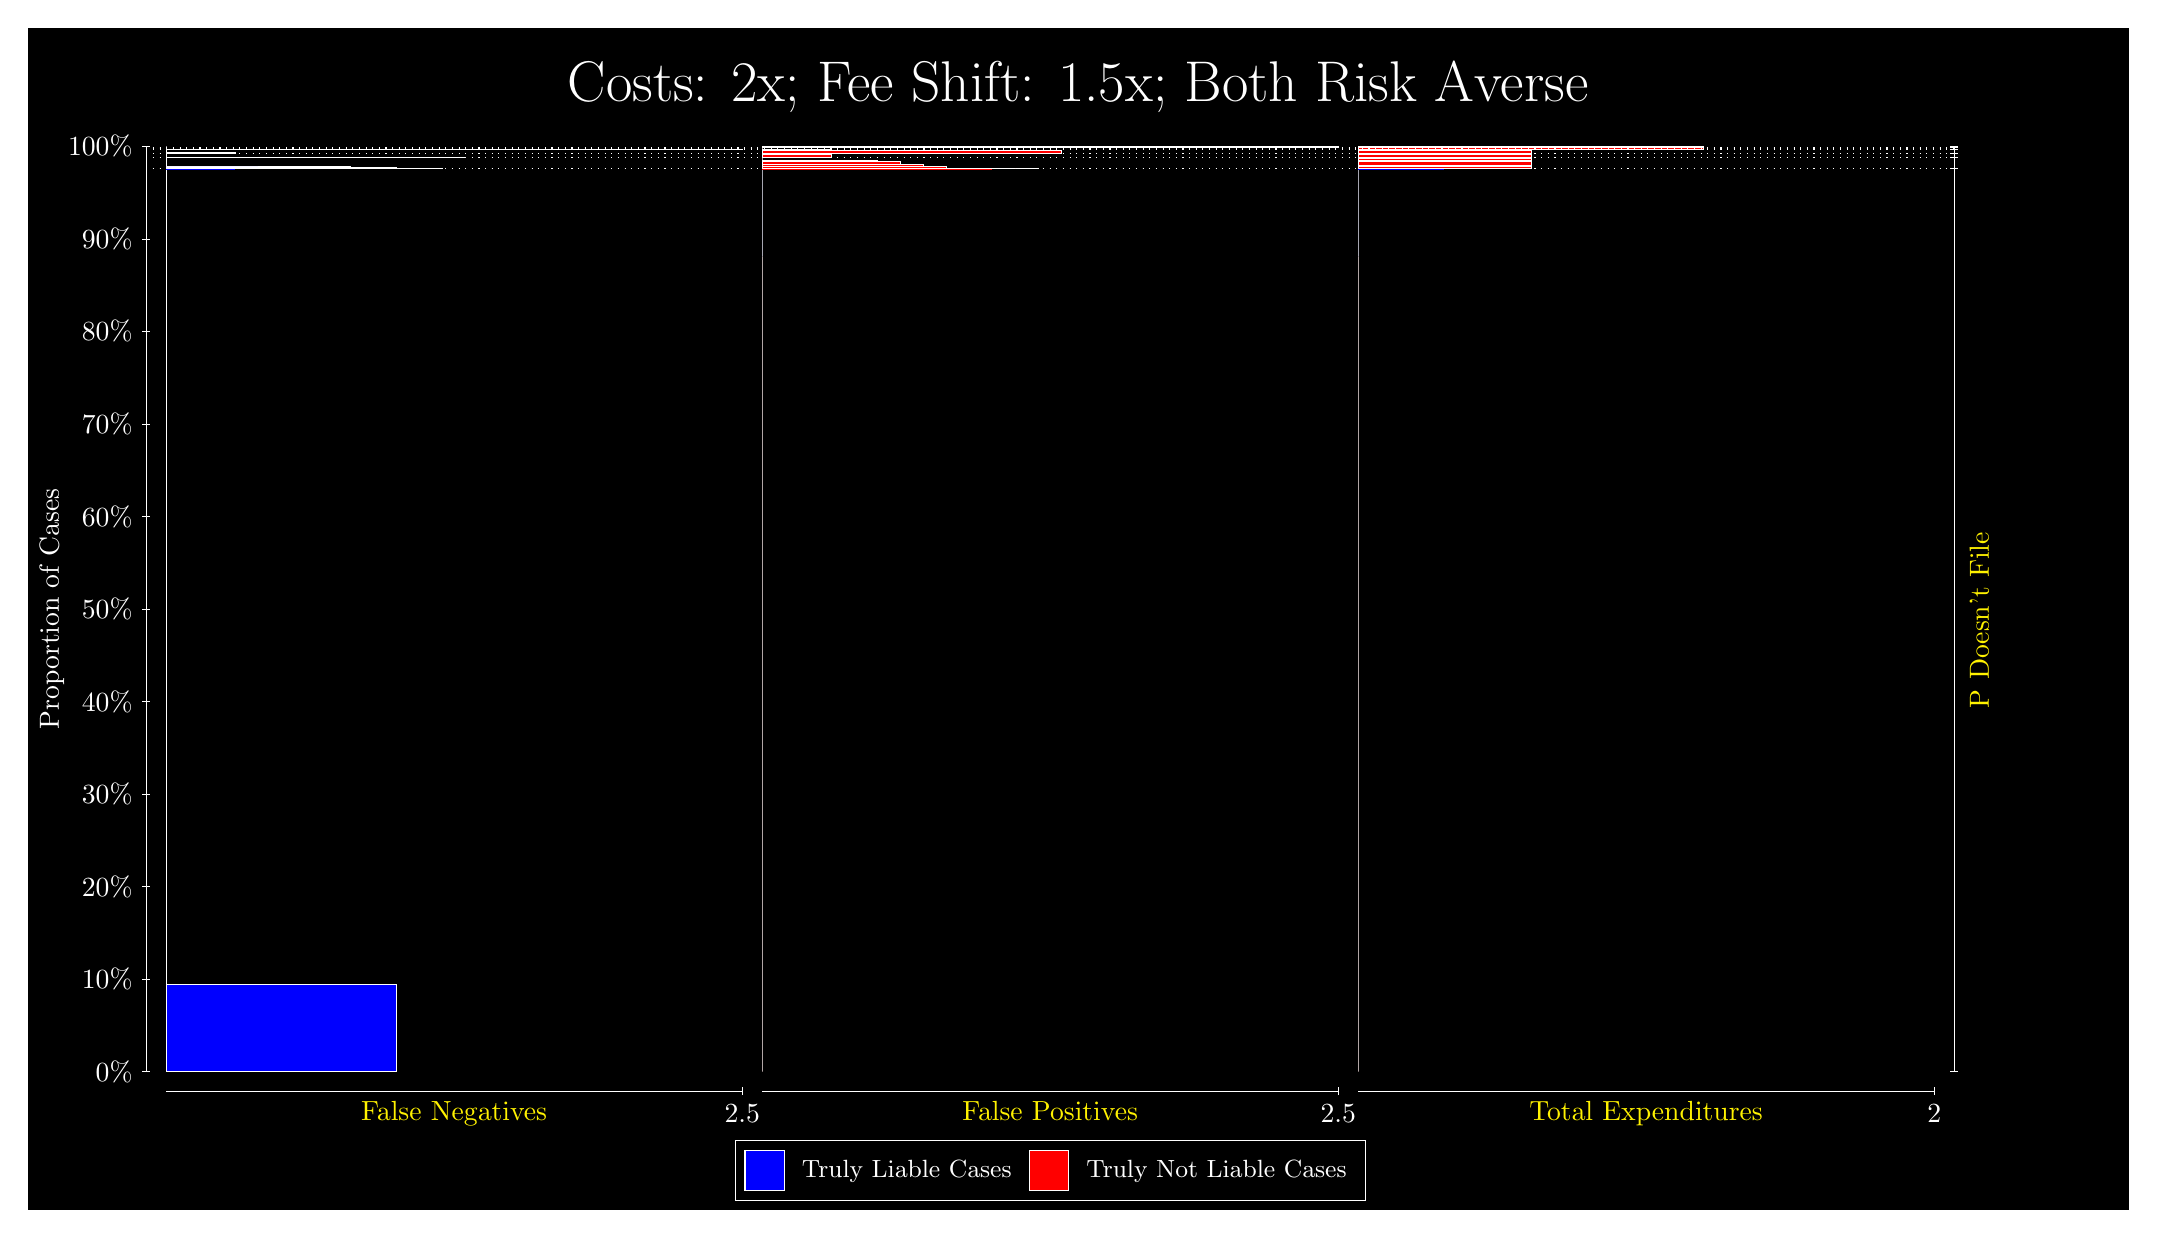
\begin{tikzpicture}
\draw[fill=black] (0,0) rectangle (26.667,15);
\draw[text=white] (0,13.5) rectangle (26.667,15) node[midway] {\huge Costs: 2x; Fee Shift: 1.5x; Both Risk Averse};
\draw[white, very thin] (1.5,1.75) -- (1.5,13.5);
\node[rotate=90, text=white, anchor=center] at (0.3, 7.625) {Proportion of Cases};
\draw[white, very thin] (1.45,1.75) -- (1.55,1.75);
\node[text=white, anchor=east] at (1.45, 1.75) {0\%};
\draw[white, very thin] (1.45,2.925) -- (1.55,2.925);
\node[text=white, anchor=east] at (1.45, 2.925) {10\%};
\draw[white, very thin] (1.45,4.1) -- (1.55,4.1);
\node[text=white, anchor=east] at (1.45, 4.1) {20\%};
\draw[white, very thin] (1.45,5.275) -- (1.55,5.275);
\node[text=white, anchor=east] at (1.45, 5.275) {30\%};
\draw[white, very thin] (1.45,6.45) -- (1.55,6.45);
\node[text=white, anchor=east] at (1.45, 6.45) {40\%};
\draw[white, very thin] (1.45,7.625) -- (1.55,7.625);
\node[text=white, anchor=east] at (1.45, 7.625) {50\%};
\draw[white, very thin] (1.45,8.8) -- (1.55,8.8);
\node[text=white, anchor=east] at (1.45, 8.8) {60\%};
\draw[white, very thin] (1.45,9.975) -- (1.55,9.975);
\node[text=white, anchor=east] at (1.45, 9.975) {70\%};
\draw[white, very thin] (1.45,11.15) -- (1.55,11.15);
\node[text=white, anchor=east] at (1.45, 11.15) {80\%};
\draw[white, very thin] (1.45,12.325) -- (1.55,12.325);
\node[text=white, anchor=east] at (1.45, 12.325) {90\%};
\draw[white, very thin] (1.45,13.5) -- (1.55,13.5);
\node[text=white, anchor=east] at (1.45, 13.5) {100\%};

\draw[white, very thin] (24.457,1.75) -- (24.457,13.5);
\draw[white, very thin] (24.407,1.75) -- (24.507,1.75);
\node[anchor=west] at (24.407, 1.75) {};
\draw[white, very thin] (24.407,13.216) -- (24.507,13.216);
\node[anchor=west] at (24.407, 13.216) {};
\draw[white, very thin] (24.407,13.218) -- (24.507,13.218);
\node[anchor=west] at (24.407, 13.218) {};
\draw[white, very thin] (24.407,13.357) -- (24.507,13.357);
\node[anchor=west] at (24.407, 13.357) {};
\draw[white, very thin] (24.407,13.413) -- (24.507,13.413);
\node[anchor=west] at (24.407, 13.413) {};
\draw[white, very thin] (24.407,13.466) -- (24.507,13.466);
\node[anchor=west] at (24.407, 13.466) {};
\draw[white, very thin] (24.407,13.487) -- (24.507,13.487);
\node[anchor=west] at (24.407, 13.487) {};
\draw[white, very thin] (24.407,13.5) -- (24.507,13.5);
\node[anchor=west] at (24.407, 13.5) {};

\draw[white, very thin, fill=blue] (1.75,1.75) rectangle (4.6775,2.8624);
\draw[white, very thin, fill=red] (1.75,2.8624) rectangle (1.75,13.216);
\draw[white, very thin, fill=blue] (1.75,13.216) rectangle (2.6283,13.217);
\draw[white, very thin, fill=red] (1.75,13.217) rectangle (1.75,13.218);
\draw[white, very thin, fill=blue] (1.75,13.218) rectangle (5.2631,13.22);
\draw[white, very thin, fill=blue] (1.75,13.22) rectangle (4.9703,13.222);
\draw[white, very thin, fill=blue] (1.75,13.222) rectangle (4.6775,13.231);
\draw[white, very thin, fill=blue] (1.75,13.231) rectangle (4.3848,13.232);
\draw[white, very thin, fill=blue] (1.75,13.232) rectangle (4.3848,13.24);
\draw[white, very thin, fill=blue] (1.75,13.24) rectangle (4.092,13.249);
\draw[white, very thin, fill=blue] (1.75,13.249) rectangle (3.7993,13.249);
\draw[white, very thin, fill=blue] (1.75,13.249) rectangle (3.5065,13.249);
\draw[white, very thin, fill=blue] (1.75,13.249) rectangle (3.2138,13.25);
\draw[white, very thin, fill=blue] (1.75,13.25) rectangle (2.921,13.25);
\draw[white, very thin, fill=red] (1.75,13.25) rectangle (1.75,13.357);
\draw[white, very thin, fill=blue] (1.75,13.357) rectangle (5.5558,13.367);
\draw[white, very thin, fill=red] (1.75,13.367) rectangle (1.75,13.413);
\draw[white, very thin, fill=blue] (1.75,13.413) rectangle (2.6283,13.427);
\draw[white, very thin, fill=red] (1.75,13.427) rectangle (1.75,13.466);
\draw[white, very thin, fill=blue] (1.75,13.466) rectangle (9.0689,13.467);
\draw[white, very thin, fill=red] (1.75,13.467) rectangle (1.75,13.487);
\draw[white, very thin, fill=red] (1.75,13.487) rectangle (1.75,13.496);
\draw[white, very thin, fill=blue] (1.75,13.496) rectangle (1.75,13.5);
\draw[white, very thin, fill=red] (9.3189,1.75) rectangle (9.3189,12.103);
\draw[white, very thin, fill=blue] (9.3189,12.103) rectangle (9.3189,13.216);
\draw[white, very thin, fill=red] (9.3189,13.216) rectangle (12.246,13.217);
\draw[white, very thin, fill=blue] (9.3189,13.217) rectangle (9.3189,13.218);
\draw[white, very thin, fill=red] (9.3189,13.218) rectangle (12.832,13.219);
\draw[white, very thin, fill=red] (9.3189,13.219) rectangle (12.539,13.219);
\draw[white, very thin, fill=red] (9.3189,13.219) rectangle (12.246,13.221);
\draw[white, very thin, fill=red] (9.3189,13.221) rectangle (11.954,13.222);
\draw[white, very thin, fill=red] (9.3189,13.222) rectangle (11.661,13.248);
\draw[white, very thin, fill=red] (9.3189,13.248) rectangle (11.368,13.27);
\draw[white, very thin, fill=red] (9.3189,13.27) rectangle (11.075,13.305);
\draw[white, very thin, fill=red] (9.3189,13.305) rectangle (10.783,13.318);
\draw[white, very thin, fill=red] (9.3189,13.318) rectangle (10.49,13.325);
\draw[white, very thin, fill=blue] (9.3189,13.325) rectangle (9.9044,13.325);
\draw[white, very thin, fill=blue] (9.3189,13.325) rectangle (9.6116,13.325);
\draw[white, very thin, fill=blue] (9.3189,13.325) rectangle (9.3189,13.357);
\draw[white, very thin, fill=red] (9.3189,13.357) rectangle (10.197,13.403);
\draw[white, very thin, fill=blue] (9.3189,13.403) rectangle (9.3189,13.413);
\draw[white, very thin, fill=red] (9.3189,13.413) rectangle (13.125,13.452);
\draw[white, very thin, fill=blue] (9.3189,13.452) rectangle (10.197,13.466);
\draw[white, very thin, fill=red] (9.3189,13.466) rectangle (9.3189,13.486);
\draw[white, very thin, fill=blue] (9.3189,13.486) rectangle (9.3189,13.487);
\draw[white, very thin, fill=red] (9.3189,13.487) rectangle (16.638,13.496);
\draw[white, very thin, fill=blue] (9.3189,13.496) rectangle (13.71,13.5);
\draw[white, very thin, fill=red] (16.888,1.75) rectangle (16.888,12.103);
\draw[white, very thin, fill=blue] (16.888,12.103) rectangle (16.888,13.216);
\draw[white, very thin, fill=red] (16.888,13.216) rectangle (17.986,13.217);
\draw[white, very thin, fill=blue] (16.888,13.217) rectangle (17.986,13.218);
\draw[white, very thin, fill=red] (16.888,13.218) rectangle (19.083,13.246);
\draw[white, very thin, fill=blue] (16.888,13.246) rectangle (19.083,13.256);
\draw[white, very thin, fill=red] (16.888,13.256) rectangle (19.083,13.311);
\draw[white, very thin, fill=blue] (16.888,13.311) rectangle (19.083,13.324);
\draw[white, very thin, fill=red] (16.888,13.324) rectangle (19.083,13.348);
\draw[white, very thin, fill=blue] (16.888,13.348) rectangle (19.083,13.357);
\draw[white, very thin, fill=red] (16.888,13.357) rectangle (19.083,13.403);
\draw[white, very thin, fill=blue] (16.888,13.403) rectangle (19.083,13.413);
\draw[white, very thin, fill=red] (16.888,13.413) rectangle (19.083,13.452);
\draw[white, very thin, fill=blue] (16.888,13.452) rectangle (19.083,13.466);
\draw[white, very thin, fill=red] (16.888,13.466) rectangle (21.279,13.486);
\draw[white, very thin, fill=blue] (16.888,13.486) rectangle (21.279,13.487);
\draw[white, very thin, fill=red] (16.888,13.487) rectangle (21.279,13.496);
\draw[white, very thin, fill=blue] (16.888,13.496) rectangle (21.279,13.5);
\draw[white, dotted] (1.5,13.216) -- (24.457,13.216);
\draw[white, dotted] (1.5,13.218) -- (24.457,13.218);
\draw[white, dotted] (1.5,13.357) -- (24.457,13.357);
\draw[white, dotted] (1.5,13.413) -- (24.457,13.413);
\draw[white, dotted] (1.5,13.466) -- (24.457,13.466);
\draw[white, dotted] (1.5,13.487) -- (24.457,13.487);
\draw[white, very thin] (1.75,1.5) -- (9.0689,1.5);
\node[text=yellow, anchor=north] at (5.4094, 1.5) {False Negatives};
\draw[white, very thin] (9.0689,1.45) -- (9.0689,1.55);
\node[text=white, anchor=north] at (9.0689, 1.45) {2.5};

\draw[white, very thin] (9.3189,1.5) -- (16.638,1.5);
\node[text=yellow, anchor=north] at (12.978, 1.5) {False Positives};
\draw[white, very thin] (16.638,1.45) -- (16.638,1.55);
\node[text=white, anchor=north] at (16.638, 1.45) {2.5};

\draw[white, very thin] (16.888,1.5) -- (24.207,1.5);
\node[text=yellow, anchor=north] at (20.547, 1.5) {Total Expenditures};
\draw[white, very thin] (24.207,1.45) -- (24.207,1.55);
\node[text=white, anchor=north] at (24.207, 1.45) {2};

\node[text=yellow, centered, rotate=90] at (24.777, 7.4828) {P Doesn't File};







\draw (12.978300999999998,1.5) node[draw=none] (baseCoordinate) {};
\begin{scope}[align=center]
        \matrix[scale=0.5, draw=white, below=0.5cm of baseCoordinate, nodes={draw}, column sep=0.1cm]{
            \node[rectangle, draw, minimum width=0.5cm, minimum height=0.5cm, fill=blue] {}; &
            \node[draw=none, font=\small, text=white] (B) {Truly Liable Cases}; &
            \node[rectangle, draw, minimum width=0.5cm, minimum height=0.5cm, fill=red] {}; &
            \node[draw=none, font=\small, text=white] (B) {Truly Not Liable Cases}; \\
            };
\end{scope}

\end{tikzpicture}
\end{document}